\documentclass[letterpaper, 10 pt, conference]{ieeeconf}
\IEEEoverridecommandlockouts
\overrideIEEEmargins
\usepackage[T1]{fontenc}
\usepackage{times,amsmath,amssymb,graphicx,booktabs,cite,url}
\usepackage[hidelinks,pdfauthor={},pdftitle={When Does Controller Target Readback Help Cartesian Demonstration Replay?}]{hyperref}
\ifdefined\pdfminorversion\pdfminorversion=5\fi
\title{\LARGE\bf When Does Controller Target Readback Help\\ Cartesian Demonstration Replay?}
\author{\phantom{Anonymous Author}}
\begin{document}
\maketitle
\thispagestyle{empty}
\pagestyle{empty}
\begin{abstract}
A robot replaying a Cartesian demonstration can observe its hand and remember every command it sent, yet still lose track of the target stored by its controller. When does reading that target improve manipulation? We derive the worst error achievable on the next bounded target write with and without a read, then compare policies on matched simulated arm trajectories. On Fetch, re-encoding displacements relative to the measured hand rescued 19 of 48 layouts after a five-step input override without a target read. On Sawyer, a hand-based observer succeeded in 140 of 144 trials. Adding 123 reads changed none of the terminal outcomes and reduced mean hand-path error by 0.039\,mm. On a simulated Panda, direct copying failed on all eight descent overrides in each of two controller modes, while hand-based reconstruction recovered all eight. During lift, reading the accumulating controller corrected a 120.32\,mm mean origin estimate error but changed its next target by only 0.026\,mm on average. Three read-only successes with coarse hand measurements did not recur on 24 new layouts. These results identify when readback can change a command and show how command limits and hand feedback constrain its value for task completion.
\end{abstract}
\begin{keywords}Motion Control, Performance Evaluation and Benchmarking.\end{keywords}

\section{Introduction}
A replay program sends a displacement to a robot arm, then discovers that the hand is behind the demonstration. If the controller adds the next displacement to the measured hand position, the program can recompute the command from that measurement. If the controller adds it to a stored target, the same measurement can be consistent with several command histories. Reading the stored target resolves its current value. Whether the robot can use that information to bring an object to its goal is a separate question (Fig.~\ref{fig:origin}).
\begin{figure}[t]
\centering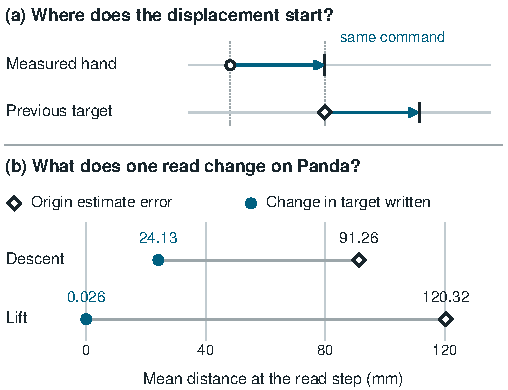
\includegraphics[width=\columnwidth]{figures/origin-readback.pdf}
\caption{(a) The same displacement starts at the measured hand or the previous target, depending on the controller. (b) At the first command after a five-step override on the accumulating Panda, the mean error in the estimated origin (open diamond) can greatly exceed the change in the target actually written after a read (filled circle). Values average eight matched layouts per phase.}\label{fig:origin}
\end{figure}
Action definitions vary across robot datasets and can affect transfer~\cite{openx2024,aljalbout2024action}. ManiSkill2 distinguishes measured and desired command references when converting demonstrations~\cite{gu2023maniskill2}. MimicGen converts target poses into bounded actions~\cite{mimicgen2023}. These methods motivate an execution question. When an applied input differs from the one recorded by the sender, which observation should a replay program use to reconstruct its next displacement?

Reference governors and reactive trajectory adaptation address command constraints and feedback during execution~\cite{governor,vochten2021}. Event-triggered control and estimation relate communication to a control or estimation objective~\cite{tabuada,trimpe}. Input acknowledgments can inform a controller about losses~\cite{schenato}, and event-triggered communication has supported cooperative manipulation~\cite{cooperative}. We examine a specific message in single-arm replay, the receiver's current Cartesian target. Its value depends on what the measured hand and submitted commands already reveal.

We derive a tight one-write error bound, then compare the same hand-based observer with and without target reads during simulated push, grasp and drawer trials. Switching the command origin on the same Panda isolates the interface from robot identity. Physical recordings and a Franka controller filter identify which telemetry could support reconstruction on hardware.
\section{What Can a Target Read Resolve?}
\subsection{The command seen by the receiving controller}
Let $x_t^\star$ and $x_t$ denote the demonstrated and replayed hand positions just before command $t$. The source command specifies a translation $a_t$ in metres after action scaling, and writes the target $g_t^\star$. The recorded hand need not have reached that target. We score the hand against the recorded hand at the same post-step time and score the target separately at the instant it is written.

Let $b_t$ be the command origin, $s$ the per-axis limits, and $C$ the workspace clip. A legal displacement $d$ writes
\begin{equation}
 F(b_t,d)=C(b_t+d),\quad -s\le d\le s .\label{eq:setter}
\end{equation}
Fetch uses the measured gripper position as $b_t$. Sawyer uses its last written target. On the source tape, Fetch's hand and command determine $g_t^\star$. On Sawyer the initial target and the commands applied during the clean demonstration determine it recursively. A replay read supplies the current \emph{destination} origin. It leaves the source tape unchanged.

To retain the lag between hand and target in the demonstration, we request $h_t=g_t^\star+k(x_t^\star-x_t)$, where $k$ is the hand feedback gain. For an origin estimate $b$, project $h_t$ onto the reachable box $[C(b-s),C(b+s)]$ to obtain $q$. Sending $d=\operatorname{clip}_{[-s,s]}(q-b)$ realizes $q$ if $b$ is the true origin and the command reaches the setter.

\subsection{A tight error floor for two compatible histories}
Suppose the observations and sent commands leave two possible origins, $b$ and $b-v$. For example, a hidden overwrite could replace $v$ by zero. Take $h=b$ and assume the workspace is locally inactive and $v$ is an admissible displacement. Sending a common $d$ incurs Euclidean errors $\|d\|_2$ and $\|d-v\|_2$. By the triangle inequality their larger value is at least $\|v\|_2/2$, attained by $d=v/2$. A program that insists on zero error for the first history must send $d=0$ and incur $\|v\|_2$ on the other. An exact read allows a different command in each history and zero error on both. The ambiguity lasts only as long as both histories remain compatible with the available observations.

We tested this construction on Sawyer's native setter at 16 reset states across push and drawer-open. We held the hand, joint positions and joint velocities fixed, separated the stored origins along one axis by 2, 5 or 8\,mm, and issued zero, midpoint and exact corrections. Across 144 matched problems (864 writes), the largest absolute difference from the predicted residual was below $10^{-10}$\,mm (Fig.~\ref{fig:ambiguity}).
\begin{figure}[t]
\centering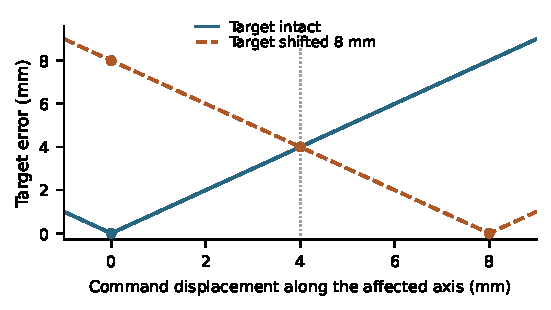
\includegraphics[width=\columnwidth]{figures/ambiguity.pdf}
\caption{One native Sawyer setter state with two origins 8\,mm apart. Lines show the predicted write errors for a shared displacement on one axis. The dots show native setter writes. A 4\,mm midpoint gives the smallest worst error without a read. Reading the origin lets the program choose the zero-error action for each history.}\label{fig:ambiguity}
\end{figure}

\input{read-value}
\section{Paired Replay Protocol}
\subsection{Demonstrations, interventions and outcomes}
For each layout, we record a scripted demonstration, restore the initial state and replay to a fixed horizon. Policies receive the source tape and measured hand positions. Gripper commands pass through unchanged. We use object state, fault labels and task predicates to construct and score the experiments. We verify initial states and source tapes across paired policies and retain failed demonstrations.

Fetch push and pick-and-place use Gymnasium-Robotics 1.4.2 and MuJoCo 3.3.7, with a 50-step horizon and 50\,mm per-axis translation scale~\cite{plappert2018fetch}. Meta-World 3.1.1 and MuJoCo 3.3.0 use 10\,mm increments relative to Sawyer's previous mocap target~\cite{yu2020metaworld,mclean2025metaworld}. We use its released push, pick-place and drawer-open experts and evaluate at step 150. Each layout undergoes four conditions: clean replay, five consecutive translations overwritten by zero, a 20\,N hand force along negative world $y$ for three steps, and both interventions. We draw onset times from steps 7--29 on Fetch and 8--65 on Sawyer. All policies in a pair share those times. Fault type and onset are hidden during ordinary replay.

The initial comparison uses 24 held-out layouts per task, or 120 layouts and 3,360 branch executions. Seven clean Fetch push demonstrations miss the task goal and remain in the sample. Follow-up comparisons use separately identified cohorts. We score the native success predicate at the \emph{last} step. For each episode the hand-path RMS error is $\sqrt{T^{-1}\sum_{t=1}^{T}\|x_t-x_t^\star\|_2^2}$. We average this error across episodes. Paired bootstrap intervals resample layouts within each task, carrying all conditions for each layout together. Equal task and intervention weights define this stress test. They have no assumed deployment frequency.

\subsection{Information supplied to each policy}
A command-history policy starts with the known origin and updates it using the commands it sends. An undetected overwrite breaks that recursion. A target read resets the estimate. In the original event policy, two consecutive hand deviations above 5\,mm trigger a read, with a ten-step cooldown and at most two reads per trial. A scheduled policy reads at steps 16 and 32 on Fetch or 50 and 100 on Sawyer. The Sawyer times and $k=0.5$ came from a development comparison of three schedules and two gains. A lower-cost variant checks the residual at the two scheduled times only.

The hand-based observer uses the recorded offset between source hand and source origin. Let $\tilde b_t$ be the live origin predicted from previous estimates and sent commands, and let $b_t^\star$ be the source origin. The correction is
\begin{equation}
 \hat b_t=C\!\left(\tilde b_t+0.25\big[x_t+(b_t^\star-x_t^\star)-\tilde b_t\big]\right).\label{eq:observer}
\end{equation}
It places the recorded offset at the current hand, blends this candidate with the prediction, and propagates the updated estimate using its next submitted command. The read and zero-read branches share this observer, including its gain. We froze it after an eight-layout development trial. It assumes access to a clean source tape, an initialized target and time-aligned hand measurements.

For the limited-resolution comparisons we delay both hand measurements and requested targets by two steps. We propagate a delayed target with submitted commands and transport the last measured hand residual along the demonstration. Only the replay's live hand is rounded to a 1 or 5\,mm grid in world coordinates. The event policy may read once after two steps above 5\,mm. Before testing new layouts at 5\,mm, we fix a read at step 41 (the median development event time) and define a second schedule by permuting the 96 development event times independently of the new motions.

\section{When Does Readback Change the Outcome?}
\subsection{Re-encoding at a measured origin}
After the five-step override, direct copying succeeded on 22 of 48 Fetch layouts. Re-encoding the desired target from the measured hand succeeded on 41 of 48, matching the number of successful source demonstrations. It rescued ten push and nine pick-and-place trials without losing any or requesting the controller target. Figure~\ref{fig:fetch} shows one rescued push. Under force alone re-encoding lost one push that direct copying completed, even though across force trials the mean hand-path RMS error fell from 0.033 to 0.005\,mm. Improving hand tracking does not ensure the cube finishes closer to its goal.
\begin{figure}[t]
\centering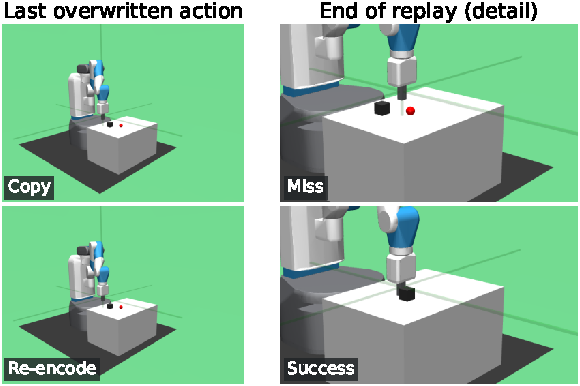
\includegraphics[width=\columnwidth]{figures/fetch-example.pdf}
\caption{Replay of the same FetchPush layout after five overwritten translations. At tick 14 the final overwrite occurs (left). At the last tick the cube is 134.4\,mm from the goal under direct copying and 23.3\,mm from it after re-encoding (right, enlarged). We show the lowest-index held-out push layout rescued by re-encoding.}\label{fig:fetch}
\end{figure}

\subsection{How much does Sawyer's hand already reveal?}
The clearest comparison holds the observer fixed and varies access to the internal target. On 36 fresh Sawyer layouts (12 per task), the hand-based observer recovered six trials lost by command history alone, with no losses. Reading on events while retaining command history recovered exactly the same six. Adding event reads to the hand-based observer changed none of the 144 paired terminal outcomes (Table~\ref{tab:observer}). The 123 extra reads reduced mean hand-path RMS error by 0.039\,mm (paired 95\% layout-bootstrap interval for the reduction, 0.012--0.068\,mm). Four push trials still failed with either observer branch.
\begin{table}[t]\centering
\caption{Sawyer policies on the same 36 layouts and four conditions per layout. Reads are total extra requests. RMS is the mean of per-episode hand-path errors.}\label{tab:observer}
\begin{tabular}{@{}lrrr@{}}\toprule
Origin estimate and read policy & Success & Reads & RMS (mm)\\\midrule
Command history only & 134/144 & 0 & 6.497\\
Command history + event & 140/144 & 112 & 2.734\\
Hand-based observer & 140/144 & 0 & 2.830\\
Observer + event & 140/144 & 123 & 2.790\\
Observer + gated fixed times & 140/144 & 32 & 2.829\\\bottomrule
\end{tabular}
\end{table}

Earlier schedule comparisons illustrate why the choice of baseline matters. With command history and hand feedback gain $k=0.5$, event and scheduled reads yielded 192/192 and 190/192 successes on push and pick-place, using 160 and 384 reads, respectively. The two event-only successes arose on a single pick-place layout, under the overwrite and combined conditions (Fig.~\ref{fig:sawyer}). The difference was 1.04 percentage points (95\% layout-bootstrap interval, 0.00--3.13). It fell short of the prespecified five-point gain with a positive lower confidence limit. The 96 drawer conditions agreed. At $k=0$, event reads succeeded on 192/192 compared with 166/192 for the scheduled reads. The larger difference applies to this weaker hand-feedback comparator.
\begin{figure}[t]
\centering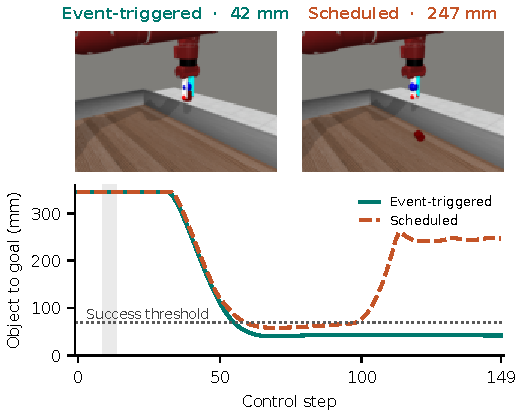
\includegraphics[width=\columnwidth]{figures/sawyer-case.pdf}
\caption{The single Sawyer pick-place layout accounting for both event-only successes against scheduled reads at $k=0.5$. During the overwrite trial both policies brought the object within 70\,mm of its goal. At the final step the event branch was 42.3\,mm away and the scheduled branch 246.7\,mm away.}\label{fig:sawyer}
\end{figure}

Checking the hand residual twice versus at every step on 36 fresh layouts gave 144/144 successes for both, with 60 versus 106 reads and 4.16 versus 3.14\,mm mean hand RMS. On a separate 36 layouts the rewrite guard~\eqref{eq:guard} admitted 658 of 12,474 proposals. Of these, 560 reached the setter, and each reduced squared write error as certified. Both guarded and unguarded branches succeeded on all 144 trials. The guard used more reads (125 versus 115) and had greater hand RMS (2.96 versus 2.64\,mm). Its guarantee is local to a delivered write.

On 24 further push and pick-place layouts, we timed overrides to begin six steps before or one step after the first pad--object contact in the source. The observer alone and a single read 0, 1, 2, 4 or 8 steps after the overwrite each achieved 48/48 across the two phases. Before the read, the mean origin error fell from 28.90\,mm at zero delay to 10.68\,mm at eight steps. The no-read and immediate-read hand RMS values were 8.02 and 7.95\,mm.

To test a trigger without access to the fault time, we compared two candidate commands computed from the available origin estimates. The policy could request once when their difference exceeded 2.5\,mm for two steps. On a separate 24-layout cohort, adding this trigger changed no terminal outcome relative to the zero-request observer. Both scored 96/96 with synchronous observations, 94/96 with a two-step delay, and 96/96 when the delayed interface also published the target every three steps. Under delay the 48 extra requests raised mean hand-path RMS from 4.429 to 4.504\,mm. The two failures without the periodic stream came from one pick-place layout.

\subsection{Changing the command origin on the same Panda}
To control for robot identity, we switched the native Cartesian controller of one simulated Panda between measured and accumulating origins in robosuite 1.5.2 (MuJoCo 3.3.7)~\cite{robosuite2020}. We used the same eight initial physical layouts in both modes and generated a clean source for each mode and layout. At 20\,Hz the source closed the gripper at step 60 and raised it at step 80. We overwrote five translations during descent (steps 35--39) or lift (80--84). One observer branch read once immediately after the scheduled override. This timing tests the effect of knowing the origin at that instant. Success required the cube center to finish more than 40\,mm above the table at step 120. All 16 sources succeeded. We retained all 192 replays, including failures.

After the descent override, direct copying failed on every layout in both modes. On the measured-origin controller, re-encoding from the current hand rescued all eight. On the accumulating controller, integration of submitted commands rescued none, whereas the hand-based observer and the observer with one read each rescued all eight. During lift every policy succeeded on all eight layouts. All terminal successes also held over the last 20 steps.
\begin{figure}[t]
\centering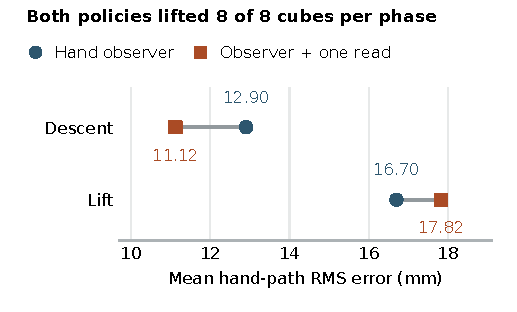
\includegraphics[width=\columnwidth]{figures/replay-comparison.pdf}
\caption{Paired replays on the accumulating Panda controller. A read after the descent override reduced mean hand-path RMS error from 12.90 to 11.12\,mm. During lift it increased the error from 16.70 to 17.82\,mm. Both observer policies lifted the cube on all eight layouts in each phase.}\label{fig:panda}
\end{figure}

The effect on the written target differed by phase. A descent read changed the next target by 24.13\,mm on average. During lift it corrected a mean origin estimate error of 120.32\,mm but changed the next target by only 0.026\,mm. Both policies had already requested maximum upward translation on every layout. Subsequent hand trajectories could still diverge (Fig.~\ref{fig:panda}).

\subsection{Three rescues with coarse hand feedback}
With two-step observation latency, unrounded and 1\,mm hand observations yielded 94/96 Sawyer successes with and without an event read on 24 push and pick-place layouts. On a 5\,mm grid the event policy achieved 94/96 versus 91/96 for the observer alone. All three extra successes came from two push layouts. The policy requested on all 96 development episodes, including all 24 clean episodes.

On 24 new layouts with the 5\,mm grid, the zero-read, event, fixed-time and permuted-time policies each succeeded on 96/96. They used 0, 94, 96 and 96 reads and had mean hand RMS errors of 6.409, 6.227, 6.293 and 6.399\,mm, respectively. The development rescues did not recur (Fig.~\ref{fig:confirm}). The ceiling in the new cohort limits inference about rarer conditions in which a read might rescue contact.

\begin{figure}[t]
\centering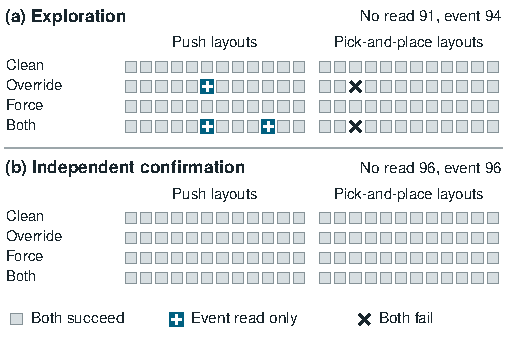
\includegraphics[width=\columnwidth]{figures/sawyer-confirmation.pdf}
\caption{Paired terminal outcomes with 5\,mm Sawyer hand observations. Each column is one layout and each row one intervention. Three event-only successes came from two development layouts. The four frozen policies each succeeded on every confirmation trial.}\label{fig:confirm}
\end{figure}

\input{discussion}
\section*{Acknowledgment}
OpenAI Codex assisted with experimental design, implementation and execution, literature checks, analysis, figure code and drafting throughout the article. The robot images in Figs.~\ref{fig:fetch} and~\ref{fig:sawyer} are native simulation renders.
\IEEEtriggeratref{7}
\bibliographystyle{IEEEtran}
\bibliography{references}
\end{document}
